\ifx\wholebook\relax \else

\documentclass{article}

\usepackage[nomarginpar
  %, margin=.5in
]{geometry}

\addtolength{\oddsidemargin}{-0.05in}
\addtolength{\evensidemargin}{-0.05in}
\addtolength{\textwidth}{0.1in}

\usepackage[en]{../prelude}

\setcounter{page}{1}

\begin{document}

\title{Deduction}

\author{刘新宇
\thanks{{\bfseries 刘新宇} \newline
  Email: liuxinyu95@gmail.com \newline}
  }

\maketitle
\fi

\markboth{Deduction}{Mathematics of Programming}

\ifx\wholebook\relax
\chapter{Deduction}
\numberwithin{Exercise}{chapter}
\fi

\epigraph{... mathematical knowledge ... is, in fact, merely verbal knowledge. ``3'' means ``2+1'', and ``4'' means ``3+1''. Hence it follows (though the proof is long) that ``4'' means the same as ``2+2''. Thus mathematical knowledge ceases to be mysterious.}{-- Bertrand Russell}

\begin{wrapfigure}{R}{0.4\textwidth}
 \centering
 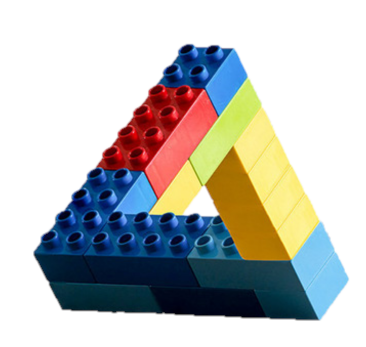
\includegraphics[scale=0.5]{img/penrose-triangle.eps}
 \captionsetup{labelformat=empty}
 \caption{Penrose triangle}
 \label{fig:Penrose-triangle}
\end{wrapfigure}

I still remember the mathematics class in high school. My teacher often wrote down a complex formula with many alphabetic symbols in the blackboard, then asked us to simplify it. Some student stood up, volunteered to do it in front of the class. Combining like terms, factorization, ... all means were attempted. It liked a magic process often led to unbelievable simple result. Of course sometimes the guy was stuck or trapped in loops, and finally saved by our teacher.

Chalk and blackboard, Such experience was unforgettable, just like happened yesterday. I was so impressive to the mythical power of reasoning. I always wanted to know more formulas, that could help me to deduce the result.

The magic is that, we even needn't care about the concrete meanings when doing the deduction. It likes building bricks, from different parts, we finally build an interesting toy. These formulas and theorems can also be combined together, and finally build an interesting result. When meet $a^2 + 2ab + b^2$, then turn it into $(a+b)^2$, just like mating two bricks. We needn't force ourselves to remind the geometric meanings for this formula when deducing it.

\begin{figure}[htbp]
\centering
\begin{tikzpicture}
\draw[fill=gray, draw=black, pattern=north west lines]
  (0, 0) rectangle (4, 4);
\filldraw[fill=white]
  (0, 0) rectangle (1, 1)
  (1, 1) rectangle (4, 4);
\path (0.5, 0.5) node {$a^2$}
      (2.5, 2.5) node {$b^2$}
      (-0.5, 0.5) node {$a$}
      (2.5, 0.5) node {$ab$}
      (4.5, 2.5) node {$b$}
      (0.5, 2.5) node {$ab$};
\path (0, -1) node (l) {}
      (2, -1) node (m) {$a + b$}
      (4, -1) node (r) {};
\draw[->] (m) -- (l);
\draw[->] (m) -- (r);
\end{tikzpicture}
\caption{Geometric illustration for $(a + b)^2 = a^2 + 2ab + b^2$}
\end{figure}

We use two examples in this chapter to demonstrate how to do deduction in programming. For every example, we'll both explain the intuitive concrete meanings, and give the purely formal deduction process. Just like the $(a+b)^2$ case, on one hand, we can explain it as the total area from two different squares and two equal rectangles; on the other hand, we can also deduce the same result step by step.

\[
\begin{array}{rcll}
(a + b)^2 & = & (a + b)(a + b) & \text{Definition of square} \\
          & = & a(a + b) + b(a + b) & \text{Distribution law for multiplication} \\
          & = & a^2 + ab + ba + b^2 & \text{Distribution law again} \\
          & = & a^2 + 2ab + b^2 & \text{Combined $ab$ and $ba$}
\end{array}
\]

\section{foldr/build fusion}

The first example is the foldr/build fusion law. In 2015, a main stream programming language Java adopted lambda expression and a set of functional tools in its 1.8 version. However, some programmer soon found the chained function calls brought elegance and expressiveness at the penalty of performance if using carelessly. One reason is the chained functions may generate excessive intermediate results. While these intermediate results are not necessary simple values, but the complete list, container, or collection of complex structures. They are thrown away after consumed by the next functions. However, the same level of new result will be generated step by step. Such produce, one time consume, thrown away, then produce again pattern happens along the function chain repeatedly, which causes computation overhead.

For example, we can define below function to examine if every element in a list satisfies a given prediction\cite{GLPJ-1993}.

\[
all(p, xs) = and(map(p, xs))
\]

Such that $all(prime, [2, 3, 5, 7, 11, 13, 17, 19, ...])$ tells if all numbers in the list are primes. However, the performance of this realization is poor. Firstly, $map(prime, xs)$ generates a list of the same length as $xs$, every element is a Boolean value [True, True, ...], indicating the corresponding number is prime or not. Then the list of Boolean values is passed to $and$ function, examine if there exists False value. Finally, both $xs$ and the Boolean list are thrown away, only one Boolean value is returned as the result.

Below is an alternative definition. It can avoid generate the intermediate Boolean list.

\[
\begin{array}{l}
all(p, xs) = h(xs) \\
  \begin{cases}
  h([]) = True \\
  h(x:xs) = p(x) \land h(xs) \\
  \end{cases}
\end{array}
\]

Although this realization does not generate intermediate result, it is neither intuitive nor elegant compare to $and(map(p, xs)$. Are there any way that has the advantage of both methods? We found some transformations satisfy such requirements, for example:

\[
map\ sqrt\  (map\ abs\ xs) = map\ (sqrt \circ abs) xs
\]

First generate a list of absolute values, then evaluate square root for every number. It is equivalent to take absolute value first, then evaluate the square root for every number in that list. Hence we have the following rule:

\be
map\ f\ (map\ g\ xs) = map\ (f \circ g)\ xs
\ee

However, there are too many rules, we can't list them all. It's not practical to apply them on a complex program. Gill, Launchbury, and Peyton Jones developed a method in 1993, starting from the basic build and folding operation, they found the pattern to optimize the chained function.

\subsection{Folding from right for list}

We defined the fold from right operation for list in chapter 1 as below:

\[
\begin{array}{l}
foldr\ \oplus\ z\ [] = z \\
foldr\ \oplus\ z\ (x:xs) = x\ \oplus\ (foldr\ \oplus\ z\ xs) \\
\end{array}
\]

It can be expanded as:

\be
foldr\ \oplus\ z\ [x_1, x_2, ..., x_n] = x_1 \oplus (x_2 \oplus (...(x_n \oplus z))...)
\ee

Many list operations can be realized by folding, for example:

\begin{enumerate}
\item Sum:

\[
sum = foldr\ +\ 0
\]

\item The $and$ function, that applies logic and for all Boolean values in a list:

\[
and = foldr\ \land\ True
\]

This is because:

\[
and\ [x_1, x_2, ..., x_n] = x_1 \land (x_2 \land (...(x_n \land True))...)
\]

\item Test if a given element belongs to a list:

\[
elem\ x\ xs\ = foldr\ (a\ b \mapsto (a = x) \lor b)\ False\ xs
\]

\item Map:

\[
\begin{array}{rcl}
map\ f\ xs & = & foldr\ (x\ ys \mapsto f(x) : ys)\ []\ xs \\
           & = & foldr\ ((:) \circ f)\ []\ xs \\
\end{array}
\]

\item Filter the elements with a given prediction:

\[
\begin{array}{rl}
filter\ f\ xs = foldr\ (x\ ys \mapsto
  \begin{cases}
    f(x): & x:ys\ \\
    \text{否则}: & ys
  \end{cases})\ []\ xs \\
\end{array}
\]

\item Concatenate two lists:

\[
xs \doubleplus ys = foldr\ (:)\ ys\ xs
\label{eq:binary-concat}
\]

This is because:

\[
[x_1, x_2, ..., x_n] \doubleplus ys = x_1 : (x_2 : (...(x_n : ys))...)
\]

\item Concatenate multiple lists:

\[
concat\ xss = foldr\ \doubleplus\ []\ xss
\]

\end{enumerate}

Actually all list operations can be realized by folding (We proved it in the F-algebra section in previous chapter), if we can simplify folding, we then can simplify all list operations.

\subsection{foldr/build fusion law}
Let's consider, what if fold from right by the cons operation (``:'') starting from an empty list [] (Nil)?

\be
foldr\ (:)\ []\ [x_1, x_2, ..., x_n] = x_1 : (x_2 : (...(x_n : []))...)
\label{eq:foldr-fixed-point}
\ee

We end up with the list itself. You may remind the fixed point introduced in previous chapter, we'll return to this topic later. In other words, if we have an operation $g$, from a starting value, for example [], and a binary operation, from example ``:'', it generates a list. We define such list construction process as $build$:

\be
build(g) = g((:), [])
\label{eq:build-definition}
\ee

Next, if we fold the list with another start value $z$ and binary operation $f$, the result is equivalent to call $g$ by replacing [] with $z$, and replacing ``(:)'' with $f$.

\be
\pmb{foldr}(f, z, \pmb{build}(g)) = g(f, z)
\ee

Written in pointless format (without parentheses and named arguments) is:

\be
\pmb{foldr}\ f\ z\ (\pmb{build}\ g) = g\ f\ z
\label{eq:foldr-build-fusion-law}
\ee

\index{foldr/build fusion law}
We named this formula {\em fuldr/build fusion law}.

Let us start from an example. Consider how to sum up all the integers from $a$ to $b$, which is $sum([a, a+1, ..., b-1, b])$. First, we need generate all the integers from $a$ to $b$. Below definition enumerates $a, a+1, a+2, ..., b-1, b$.

\[
range(a, b) =
\begin{cases}
a > b: & [] \\
\text{otherwise}: & a : range(a+1, b) \\
\end{cases}
\]

Such that $range(1, 5)$ builds the list [1, 2, 3, 4, 5]. Sum up the enumerated list gives the answer.

\[
sum(range(a, b))
\]

Next, we extract the start value [] and the binary operation (:) out as parameters:

\[
range'(a, b, \oplus, z) =
  \begin{cases}
  a > b: & z \\
  \text{otherwise}: & a \oplus range'(a+1, b, \oplus, z) \\
  \end{cases}
\]

We can further Curry the last two arguments of $range'$.

\[
range'\ a\ b = f\ c \mapsto
  \begin{cases}
  a > b: & c \\
  \text{otherwise}: & f\ a\ (range' (a+1)\ b\ f\ c) \\
  \end{cases}
\]

Now we can redefine $range$ with $range'$ and $build$:

\[
range(a, b) = build(range'(a, b))
\]

Next, we simplify the sum with the fusion law.

\[
\begin{array}{rcll}
sum(range(a, b)) & = & sum(build(range'(a, b))) & \text{substitute} \\
  & = & \pmb{foldr}\ (+)\ 0\ (\pmb{build}\ (range'\ a\ b)) & \text{define sum with foldr} \\
  & = & range'\ a\ b\ (+)\ 0 & \text{fusion law} \\
\end{array}
\]

It gives the simplified result, which avoid generating the intermediate list, hence optimize the algorithm. Let's see how this result expands:

\[
range'\ a\ b\ (+)\ 0 =
  \begin{cases}
  a > b: & 0 \\
  \text{otherwise}: & a + range'(a+1, b, (+), 0) \\
  \end{cases}
\]

\subsection{build forms for list}

To leverage fusion law conveniently, we can rewrite the common functions that generate list in the form of $build...foldr$. Such that when composite with folding, we can simplify $\pmb{foldr}...(\pmb{build}...foldr)$ with fusion law.

\begin{enumerate}
\item The simplest one is to generate an empty list.

\[
[] = build\ (f\ z \mapsto z)
\]

We can substitute it with the definition (\ref{eq:build-definition}) of $build$ to proof this result.

\begin{proof}
\bre
build\ (f\ z \mapsto z) & = & (f\ z \mapsto z)\ (:)\ [] & \text{definition of } build \\
  & = & (:)\ [] \mapsto [] & \beta-\text{reduction, see chapter 2} \\
  & = & [] & \\
\ere
\end{proof}

\item The next one is $cons$ operation, which links an element to a list.

\[
x : xs = build\ (f\ z \mapsto f\ x\ (foldr\ f\ z\ xs))
\]

Let us verify it.

\begin{proof}
\blre
  & build\ (f\ z \mapsto f\ x\ (foldr\ f\ z\ xs)) & \\
= & (f\ z \mapsto f\ x\ (foldr\ f\ z\ xs))\ (:)\ [] & \text{definition of } build \\
= & x : (foldr\ (:)\ []\ xs) & \beta-\text{reduction} \\
= & x : xs & \text{By (\ref{eq:foldr-fixed-point}), the fixed point of folding} \\
\elre
\end{proof}

\item List concatenation:

\[
xs \doubleplus ys = build\ (f\ z \mapsto foldr\ f\ (foldr\ f\ z\ ys)\ xs)
\]

\begin{proof}
\blre
  & build\ (f\ z \mapsto foldr\ f\ (foldr\ f\ z\ ys) xs) & \\
= & (f\ z \mapsto foldr\ f\ (foldr\ f\ z\ ys)\ xs)\ (:)\ [] & build \text{的定义} \\
= & foldr\ (:)\ (foldr\ (:)\ []\ ys)\ xs & \beta-\text{规约} \\
= & foldr\ (:)\ ys\ xs & \text{对内层用叠加的不动点} \\
= & xs \doubleplus ys & \text{由(\ref{eq:binary-concat}),列表的连接} \\
\elre
\end{proof}

\end{enumerate}

For the rest examples, we only give the final result and leave the proof as exercises.

\begin{enumerate}
\setcounter{enumi}{3}
\item Concatenate multiple lists.
\[
concat\ xss = build\ (f\ z \mapsto foldr\ (xs\ x \mapsto foldr\ f\ x xs)\ xss)
\]

\item Map.

\[
map\ f\ xs = build\ (\oplus\ z \mapsto foldr\ (y\ ys \mapsto (f\ y) \oplus ys)\ z\ xs)
\]

\item Filter.

\[
filter\ f\ xs = build\ (\oplus\ z \mapsto foldr\ (x\ xs' \mapsto
  \begin{cases}
    f(x): & x \oplus xs' \\
    \text{否则}: & xs' \\
  \end{cases})\ z\ xs) \\
\]

\item Generate an infinite long list of the same element.

\[
repeat\ x = build\ (\oplus\ z \mapsto let\ r = x \oplus r\ in\ r)
\]

\end{enumerate}

\subsection{Reduction with the fusion law}

Empowered by the fusion law, we are ready to simplify varies of computation. The first example is $all(p, xs) = and(map(p, xs))$, which was mentioned at the begining of this chapter.

\begin{example}
\normalfont
First, we express $and$ in folding form, then turn $map$ into its build form, and apply fusion law to do the reduction.

\bre
all(p, xs) & = & and(map(p, xs)) & \text{definition} \\
  & = & foldr\ \land\ True\ map(p, xs) & \text{folding form of } and \\
  & = & \pmb{foldr}\ \land\ True\ \pmb{build}\ (\oplus\ z \mapsto & \\
  &   & \quad \quad foldr\ (x\ ys \mapsto p(x) \oplus ys)\ z\ xs) & \text{build form of } map\\
  & = & (\oplus\ z \mapsto foldr\ (x\ ys \mapsto p(x) \oplus ys)\ z\ xs)\ \land\ True & \text{fusion law} \\
  & = & foldr\ (x\ ys \mapsto p(x) \land ys)\ True\ xs & \beta-\text{reduction} \\
\ere

We can define a helper function $first$, which applies a given function $f$ to the first element of a pair.

\[
(first\ f)\ x\ y = f(x)\ y
\]

Then we can further simplify $all$ to:

\[
all\ p = foldr\ (\land) \circ (first\ p)\ True
\]

\end{example}

\begin{example}
\normalfont
The second example is to concatenate multiple words together and interpolate them with spaces, such that they form a sentence. This text manipulation process is often called $join$. For illustration purpose, we add an additional space at the end of the sentence. A typical definition is as below:

\[
join(ws) = concat(map(w \mapsto w \doubleplus ['\ '], ws))
\]

This definition is straightforward. It first uses map to append a space to every word, and output a new list of words; then concatenates the list to a string. However, its performance is poor. Appending at the end of a word is an expensive operation. It need move from the head to the tail of every word first, then do the string concatenation. How many words there are, how long the new list will be. This intermediate words list is thrown away finally. Let's optimize it with the fusion law.

\[ \begin{array}{rl}
  & join(ws) \\
  & \{\text{definition} \} \\
= & concat(map(w \mapsto w \doubleplus ['\ '], ws)) \\

  & \{\text{build form of } concat\} \\
= & build\ (f\ z \mapsto \\
  & \quad foldr\ (x\ y \mapsto foldr\ f\ y\ x)\ z\ map(w \mapsto w \doubleplus ['\ '], ws)) \\

  & \{\text{build form of } map\} \\
= & build\ (f\ z \mapsto \\
  & \quad \pmb{foldr}\ (x\ y \mapsto foldr\ f\ y\ x)\ z\ (\pmb{build}\ (f'\ z' \mapsto \\
  & \quad \quad foldr\ (w\ b \mapsto f'\ (w \mapsto w \doubleplus ['\ '])\ b)\ z'\ ws))) \\

  & \{\text{fusion law}\} \\
= & build\ (f\ z \mapsto \\
  & \quad foldr\ (w\ b \mapsto (x\ y \mapsto foldr\ f\ y\ x)\ (w \doubleplus ['\ '])\ b)\ z\ ws) \\

  & \{\beta-\text{reduction}x, y\} \\
= & build\ (f\ z \mapsto \\
  & \quad foldr\ (w\ b \mapsto foldr\ f\ b\ (w \doubleplus ['\ ']))\ z\ ws) \\

  & \{\text{build form of } \doubleplus \} \\
= & build\ (f\ z \mapsto \\
  & \quad foldr\ (w\ b \mapsto \\
  & \quad \quad \pmb{foldr}\ f\ b\ (\pmb{build}\ (f'\ z' \mapsto \\
  & \quad \quad \quad foldr\ f'\ (foldr\ f'\ z'\ ['\ '])\ w)))\ z\ ws) \\

  & \{\text{fusion law}\} \\
= & build\ (f\ z \mapsto \\
  & \quad foldr\ (w\ b \mapsto \\
  & \quad \quad foldr\ (foldr\ f\ b\ ['\ '])\ w)\ z\ ws) \\

  & \{\text{substitute $(:)$ and $[]$ in the definition of $build$}\} \\
= & foldr\ (w\ b \mapsto foldr\ (:)\ \pmb{(foldr\ (:)\ b\ ['\ '])}\ w)\ []\ ws \\

  & \{\text{evaluate to bold part}\} \\
= & foldr\ (w\ b \mapsto foldr\ (:)\ ('\ ' : b)\ w)\ []\ ws \\
\end{array} \]

The final reduced result is:

\[
join(ws) = foldr\ (w\ b \mapsto foldr\ (:)\ ('\ ' : b)\ w)\ []\ ws
\]

We can further expand the folding operation to obtain a definition with both good readability and performance.

\[
\begin{array}{l}
\begin{cases}
join\ [] = [] \\
join\ (w:ws) = h\ w \\
\end{cases} \\
\text{where}: \begin{cases}
             h\ [] = '\ ' : join\ ws \\
             h\ (x:xs) = x : h\ xs \\
             \end{cases} \\
\end{array}
\]

\index{concatMap} \index{flatMap}
Because $concat \circ map(f)$ is very common, many programming environments provide it in the optimized way as we deduced\footnote{For example, \texttt{concatMap} in Haskell, and \texttt{flatMap} in Java and Scala.}.
\end{example}

Although the second example demonstrates the power of fusion law, it also exposes a problem. The reduction process is complex and error prone, with plenty of repeated similar steps. It is exactly a typical case that machine performs better than human beings. Some programming environments have the fusion law built in the compiler\cite{GLPJ-1993}. What we need is to define the common list operations in the build...foldr form, then the rest boring work can be handled by machine. The compiler will help us reducing to optimized program, that avoid thrown away intermediate results and redundant recursions\footnote{Haskell standard library for example, provides most list functions in build...foldr form.}. As time goes on, more and more compilers will support this optimization tool.

\subsection{Type constraint}

Whenever we develop an abstraction tool, we should consider its application scope, understand when it will be invalid. For the fusion law, consider the below contradict results:

\blre
  & \pmb{foldr}\ f\ z\ (\pmb{build}\ (c\ n \mapsto [0])) & \\
= & (c\ n \mapsto [0])\ f\ z & \text{fusion law} \\
= & [0] & \beta-\text{reduction} \\
\elre

On the other hand:

\blre
  & foldr\ f\ z\ (build\ (c\ n \mapsto [0])) & \\
= & foldr\ f\ z\ ((c\ n \mapsto [0])\ (:)\ []) & \text{definition of } build \\
= & foldr\ f\ z\ [0] & \beta-\text{reduction} \\
= & f(0, z) & \text{expand foldr} \\
\elre

Obviously that $f(0, z)$ is not identical to $[0]$, even their types are not same\footnote{Unless the extreme case that $f = (:), z = []$.}. The reason that leads to this contradiction is because $(c\ n \mapsto [0])$ is not a function that builds result of $c$ and $n$. It tells us, the fusion law $foldr\ f\ z\ (build\ g) = g\ f\ z$, has type constraint for $g$. Its first argument can be $c$ or $f$, actually, it accepts a polymorphic binary operation $\forall A. \forall B.\ A \times B \to B$; The second argument is the start value of a polymorphic type $B$, the result type is also $B$. Write the binary operation in Curried form, we obtain the following type constraint for $g$.

\[
g : \forall A. (\forall B. (A \to B \to B) \to B \to B)
\]

In the above example that causes contradict results, the type is $\forall A. (\forall B. (A \to B \to B) \to B \to [Int])$. It does not satisfy the constraint. The corresponding result constraint for $build$ is:

\[
build : \forall A. (\forall B. (A \to B \to B) \to B \to B) \to \mathbf{List}\ A
\]

\index{rank-2 type polymorphic}
Because there are two polymorphic types $A$ and $B$, it is called rank-2 type polymorphic.

\subsection{Fusion law in category theory}
\index{短路融合(shortcut fusion}
叠加——构建融合律可以用范畴理论推导出来并进行扩展。一旦把范畴论作为理论工具,人们就发现叠加——构建融合仅仅是众多种融合规则中的一个。现在这些规则统一被称为“短路融合”(shortcut fusion)。它们在编译器优化,程序库优化中发挥了重要的作用。我们无法在这一章中对它们做全面的介绍。读者可以参考\cite{Hinze-Harper-James-2010}深入了解短路融合的理论和实践方法。

在上一章中,我们介绍了F-代数,特别是初始代数和向下态射。由于初始代数是起始对象,所以它到任何其他代数都有唯一的箭头。如下图所示:

\begin{center}
\begin{tikzpicture}
  \matrix (m) [matrix of math nodes,
               row sep=3em, column sep=3em, minimum width=2em]{
    \mathbf{F} I  & I \\
    \mathbf{F} A  & A \\};
  \path[-stealth]
    (m-1-1) edge node [above] {$i$} (m-1-2)
    (m-1-1) edge node [left] {$\mathbf{F} \lbb a \rbb$} (m-2-1)
    (m-1-2) edge node [right] {$\lbb a \rbb$}  (m-2-2)
    (m-2-1) edge node [below] {$a$} (m-2-2);
\end{tikzpicture}
\end{center}

从初始代数$(I, i)$到另一代数$(A, a)$的箭头可以通过向下态射$\lbb a \rbb$来表示。如果还存在一个不同的F-代数$(B, b)$对象,并且有从$A$到$B$的箭头$A \arrowto{h} B$,就可以在上面的范畴图下方把$(B, b)$也画出:

\begin{center}
\begin{tikzpicture}
  \matrix (m) [matrix of math nodes,
               row sep=3em, column sep=3em, minimum width=2em]{
    \mathbf{F} I & I \\
    \mathbf{F} A & A \\
    \mathbf{F} B & B \\};
  \path[-stealth]
    (m-1-1) edge node [above] {$i$} (m-1-2)
    (m-1-1) edge node [left] {$\mathbf{F} \lbb a \rbb$} (m-2-1)
    (m-1-2) edge node [right] {$\lbb a \rbb$}  (m-2-2)
    (m-2-1) edge node [below] {$a$} (m-2-2)
    (m-3-1) edge node [below] {$b$} (m-3-2)
    (m-2-1) edge node [left] {$\mathbf{F}(h)$} (m-3-1)
    (m-2-2) edge node [right] {$h$} (m-3-2);
\end{tikzpicture}
\end{center}

但由于$(I, i)$是起始对象,所以它到$(B, b)$也必然存在唯一的箭头。由此可知,必然存在从$I$到$B$的箭头,可以用向下态射$\lbb b \rbb$表示出来。如下图:

\begin{center}
\begin{tikzpicture}
  \matrix (m) [matrix of math nodes,
               row sep=3em, column sep=3em, minimum width=2em]{
    \mathbf{F} I & I & \\
    \mathbf{F} A & A & \lbb b \rbb \\
    \mathbf{F} B & B & \\};
  \path[-stealth]
    (m-1-1) edge node [above] {$i$} (m-1-2)
    (m-1-1) edge node [left] {$\mathbf{F} \lbb a \rbb$} (m-2-1)
    (m-1-2) edge node [right] {$\lbb a \rbb$}  (m-2-2)
    (m-2-1) edge node [below] {$a$} (m-2-2)
    (m-3-1) edge node [below] {$b$} (m-3-2)
    (m-2-1) edge node [left] {$\mathbf{F}(h)$} (m-3-1)
    (m-2-2) edge node [right] {$h$} (m-3-2);
  \draw[-stealth]
    (m-1-2) .. controls (m-2-3) .. (m-3-2);
\end{tikzpicture}
\end{center}

从这个范畴图可以看出,如果存在$h$,则下面那个小正方形可交换。这等价于说从$I$经由$A$到$B$相当于从$I$直接到$B$。这就是初始代数的融合律。记为:

\be
\begin{array}{rcl}
A \arrowto{h} B \Rightarrow h \circ \lbb a \rbb = \lbb b \rbb
& \iff &
h \circ a = b \circ \mathbf{F}(h) \\
\end{array}
\ee

初始代数的融合律意味这什么呢?在上一章中,我们发现向下态射可以将非递归的计算,转换成在递归结构上的叠加计算。例如,当函子$\mathbf{F}$是$\mathbf{ListF}A$(其中$A$是给定的对象)时,箭头$a = f + z$(加号表示余积),而初始箭头$i = (:) + []$,向下态射$\lbb a \rbb = foldr(f, z)$。如果记$b = c + n$,则融合律可以写成:

\[
h \circ foldr(f, z) = foldr(c, n)
\]

它说明叠加之后再进行变换可以化简为单一的叠加。1995年,高野秋彦和梅耶(Meijer)进一步将向下态射$\lbb a \rbb$抽象成从$a$构造某种代数结构$g\ a$,这样融合律就可以推广为\cite{Takano-Meijer-1995}:

\be
A \arrowto{h} B \quad \Rightarrow \quad h \circ g\ a = g\ b
\ee

\index{酸雨定律} \index{砍伐定律(deforestation)}
这一推广的融合律被称为“酸雨定律”\footnote{由于融合律能够消除不必要的中间结果,所以最早被称为“砍伐定律”(deforestation)。而推广的融合律被幽默地称为酸雨定律(acid rain law)。}。另一方面,由于存在从初始代数$I$到$A$的箭头:$I \arrowto{\lbb a \rbb} A$,所以将$\lbb a \rbb$代入酸雨定律左侧的$h$,并且用$i$替换酸雨定律中的$a$,用$a$替换酸雨定律中的$b$,我们有:

\be
I \arrowto{\lbb a \rbb} A \quad \Rightarrow \quad \lbb a \rbb \circ g\ i = g\ a
\ee

具体到列表的例子,把$\lbb a \rbb$代换为$foldr(f, z)$;把初始代数$i$代换为列表的初始代数$(:) + []$;定义$build(g) = g\ (:)\ []$,并代入酸雨定律左侧,就得到了列表的叠加——构建融合律:

\blre
& \lbb a \rbb \circ g\ i = g\ a & \text{酸雨定律} \\

\Rightarrow &
foldr\ f\ z\ (g\ i) = g\ a & \text{列表的向下态射是叠加} \\

\Rightarrow &
foldr\ f\ z\ (g\ (:)\ []) = g\ a & \text{列表的初始代数$i$是$(:), []$} \\

\Rightarrow &
foldr\ f\ z\ (g\ (:)\ []) = g\ f\ z & \text{用$f, z$替换$a$} \\

\Rightarrow &
\pmb{foldr}\ f\ z\ (\pmb{build}\ g) = g\ f\ z & \text{反向用$build$的定义} \\
\elre

这样我们就用范畴论证明了叠加——构建融合律\cite{Hinze-Harper-James-2010}。

\begin{Exercise}
\Question{验证从左侧叠加也可以表示为$foldr$:
\[
foldl\ f\ z\ xs = foldr\ (b\ g\ a \mapsto g\ (f\ a\ b))\ id\ xs\ z
\]}
\Question{证明以下列表的构建——叠加形式:
\[
\begin{array}{l}
concat\ xss = build\ (f\ z \mapsto foldr\ (xs\ x \mapsto foldr\ f\ x xs)\ xss) \\
map\ f\ xs = build\ (\oplus\ z \mapsto foldr\ (y\ ys \mapsto (f\ y) \oplus ys)\ z\ xs) \\
filter\ f\ xs = build\ (\oplus\ z \mapsto foldr\ (x\ xs' \mapsto
  \begin{cases}
     f(x): & x \oplus xs' \\
    \text{否则}: & xs' \\
  \end{cases})\ z\ xs) \\
repeat\ x = build\ (\oplus\ z \mapsto let\ r = x \oplus r\ in\ r) \\
\end{array}
\]
}
\Question{利用融合律化简快速排序算法:
\[
\begin{cases}
qsort\ [] = [] \\
qsort\ (x:xs) = qsort\ [a | a \in xs, a \leq x] \doubleplus [x] \doubleplus qsort\ [a | a \in xs, x < a] \\
\end{cases}\]
提示:将ZF表达式\footnote{全称为“策梅罗——弗兰克尔表达式”。指集合论中$\{f(x) | x \in X, p(x), q(x), ...\}$这样的集合构建表达式。我们在下一章介绍无穷和集合论时会再次遇到它。}转换为$filter$。}
\Question{利用范畴论验证融合律的类型限制。提示:考虑向下态射的类型。}
\end{Exercise}

\section{巧算100}

我们举的第二个例子来自伯德的《函数式算法珠玑》中的第6章\cite{Bird-2010}。高德纳在《计算机程序设计的艺术》卷4中给出了一道练习题\cite{Knuth-TAOCP-2006}:把1到9这九个数字写成一行:1 2 3 4 5 6 7 8 9。只允许在这些数字之间添上加号和乘号,不许用括弧。如何使得最后的得数恰好是100?

例如:

\[
12 + 34 + 5 \times 6 + 7 + 8 + 9 = 100
\]

这看起来像是一道小学生的数学竞赛题目。如果要求找到所有可能的解法,就是一道编程趣题。最简单直接的方法,就是利用计算机进行穷举,每两个数字间一共有三种选择:1)什么都不插入;2)插入加号;3)插入乘号。由于九个数字间一共有8个空,所以共有$3^8 = 6561$种方法。我们只要让计算机逐一检查这6561种方案,看看哪些最终得100就可以了。

\subsection{穷举法}

我们先把一个由数字、加法、乘法组成的式子定义出来。考虑刚才的算式:

\[
12 + 34 + 5 \times 6 + 7 + 8 + 9
\]

由于先乘除后加减,我们可以把它看作由加号分割的若干子算式。所以上述算式等价于:

\[
sum [12, 34, 5 \times 6, 7, 8, 9]
\]

这样我们定义一个算式是由加号分割的若干子算式$t_1 + t_2 + ... + t_n$。即$expr = [t_1, t_2, ..., t_n]$:

\lstset{frame = none}
\begin{lstlisting}
type Expr = [Term]
\end{lstlisting}

具体到每个子算式,我们可以把它看作由乘号分割的若干因子,例如$5 \times 6 = product [5, 6]$。如果是单一的数,例如$34$,我们仍然可以把它看作$34 = product [34]$。这样我们就可以定义由因子组成的子算式$f_1 \times f_2 \times ... \times f_m$。即$term = [f_1, f_2, ..., f_m]$:

\begin{lstlisting}
type Term = [Factor]
\end{lstlisting}

最终,每个因子都可以看作若干数字组成的整数,例如由两个数字组成的34,或仅有一个数字的5。也就是说$factor = [d_1, d_2, ..., d_k]$:

\begin{lstlisting}
type Factor = [Int]
\end{lstlisting}

从若干数字求得整数是一个叠加的过程,例如$[1, 2, 3] \Rightarrow (((1 \times 10) + 2) \times 10) + 3$。我们可以将其定义为一个函数:

\[
dec = foldl\ (n\ d \mapsto n \times 10 + d)\ 0
\]

穷举法的思路是针对每一个可能的算式,计算并检查它是否得100。为此,我们需要定义一个函数,求出一个算式的值。根据算式的定义,我们需要递归地求出每个子算式(term)的值,然后将其累加起来;为了求每个子算式的值,需要递归地求出每个因子的值,然后再累乘起来;为了求每个因子的值,需要对每个因子使用$dec$函数。

\[
eval = sum \circ map\ (product \circ (map\ dec))
\]

明显这一定义可以用上一节介绍的融合律进行优化,我们把具体的推导过程留作练习。最终的优化结果如下:

\[
eval = foldr\ (t\ ts \mapsto (foldr\ ((\times) \circ fork(dec, id))\ 1\ t) + ts)\ 0
\]

从这一结果可以写出一个可读性与性能都更好的定义:

\[
\begin{cases}
eval\ [] = 0 \\
eval (t:ts) = product\ (map\ dec\ t) + eval(ts) \\
\end{cases}
\]

根据这一定义,如果算式为空,则其值为0;否则我们取出第一个子算式,将其中的每个因子求出并乘到一起。然后再加上剩余子算式的求值结果。这样在使用穷举法时,对每个可能的算式,我们都用$eval$求值。留下所有等于100的算式。即:

\[
filter\ (e \mapsto eval(e) == 100)\ es
\]

其中$es$是所有从1到9能够组成的算式的集合。如何产生这个集合呢?我们从空集合开始,然后每次从1到9中取出一个数字,看看能扩展出哪些合法的算式。首先,从空集合和唯一的数字$d$只能构造出一个算式:$[[[d]]]$。最内层是由数字$d$构成的唯一因子$fact = [d]$;然后是由这个因子构成的子算式$term = [fact] = [[d]]$,这个唯一的子算式构成的完整算式是$[term] = [[fact]] = [[[d]]]$。我们可以把这一构造过程定义为:

\[
expr(d) = [[[d]]]
\]

接下来,考虑一般情形。我们的策略是从右侧开始,不断取出数字9, 8, 7, ...来扩展算式。假设我们已经用数字构造了一个算式集合$[e_1, e_2, ..., e_n]$,此时如果取出下一个数字$d$,如何扩展出所有的合法算式呢?我们在本节的开头说过,每两个数字间一共由三种选择:1)什么都不插入;2)插入加号;3)插入乘号。我们来看看对于算式集合中的任意$e_i$这三种选择的含义分别是什么。将$e_i$展开表示成若干子算式的和$e_i = t_1 + t_2 + ...$,其中第一个子算式$t_1$表示为若干因子的积$t_1 = f_1 \times f_2 \times ...$。

\begin{enumerate}
\item 什么都不插入意味着将数字$d$直接添加到$e_i$的第一个子算式中的第一个因子的前面。这样由$d:f_1$组成一个新的因子。例如$e_i$是算式$8 + 9$,数字$d$是7,将7写在$8+9$的前面而什么符号都不插入,这样就得到新算式$78 + 9$;
\item 插入乘号意味着用数字$d$构成一个因子$[d]$,然后将它添加到$e_i$中第一个子算式的前面。这样由$[d]:t_1$组成一个新的子算式。具体到$8 + 9$这个例子,我们把7写在它的前面,然后在7和8之间插入一个乘号,这样就得到新算式$7 \times 8 + 9$;
\item 插入加号意味着用数字$d$构成一个子算式$[[d]]$,然后将将它添加到$e_i$的最前面,组成新的算式$[[d]]:e_i$。具体到$8 + 9$这个例子,我们把7写在它的前面,然后在7和8之间插入一个加号,这样就得到新算式$7 + 8 + 9$;
\end{enumerate}

把这三种情形转换为定义就得到了下面的函数:

\lstset{frame = none}
\begin{lstlisting}
add d ((ds:fs):ts) = [((d:ds):fs):ts,
                      ([d]:ds:fs):ts,
                      [[d]]:(ds:fs):ts]
\end{lstlisting}

其中算式$e_i$被写成了$(ds:fs):ts$的形式,$e_i$中的第一个子算式是$ds:fs$,第一个子算式中的第一个因子是$ds$。这样,从每个已有的算式,我们都可以扩展出3个新算式。而对于算式列表$[e_1, e_2, ..., e_n]$,只要分别对每个算式扩展,然后将结果连接到一起就可以了。这恰恰就是上一节我们介绍过的$concatMap$:

\[
\begin{cases}
extend\ d\ [] = [expr(d)] \\
extend\ d\ es = concatMap\ (add\ d)\ es
\end{cases}
\]

这样我们就得到了穷举法的完整定义:

\be
filter\ (e \mapsto eval(e) == 100)\ (foldr\ extend\ [1..9])
\label{eq:puzzle100-basic}
\ee

\subsection{改进}

我们能改进这个穷举法么?观察用1到9这些数字从右向左穷举算式的过程。首先我们写下数字9,在添加数字8时,可能产生3个算式,分别是:89,$8 \times 9 = 72$,和8 + 9 = 17。接下来添加7,算式789显然大于100,可以立即丢弃。并且我们确信任何在789左侧扩展出的新算式也都不可能等于100,因此也可以丢弃。这样就避免了无谓的计算。同样$7 \times 89$也大于100,可以丢弃并停止向左扩展。只有7+89是可能的候选算式。接下来我们扩展出$78 \times 9$,由于它大于100,因此被丢弃并停止扩展……

通过这一过程,我们发现,可以一边扩展算式,一边计算当前算式的值。只要超过100就丢弃并停止从这一候选算式向左继续扩展。整个过程就像一棵不断生长的树,只要树枝代表的算式超过100,就砍掉树枝,停止这一分支的生长。

\begin{figure}[htbp]
\centering
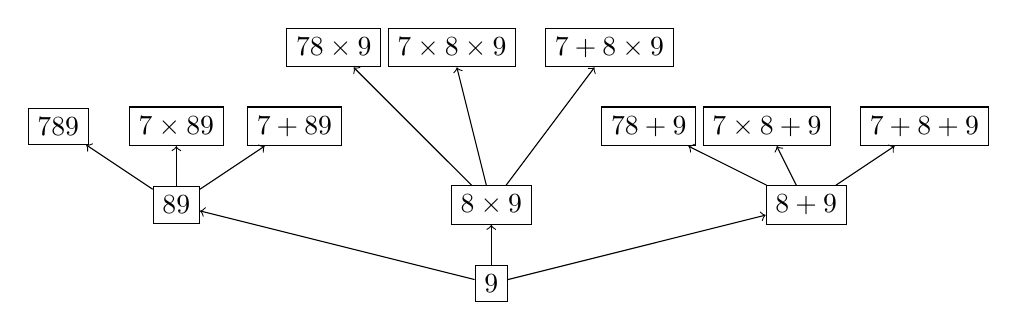
\begin{tikzpicture}
\path (0, 0)  node[rectangle, draw] (9) {9}
      (-4, 1) node[rectangle, draw] (89) {89}
      (0, 1)  node[rectangle, draw] (8x9) {$8 \times 9$}
      (4, 1)  node[rectangle, draw] (8+9) {$8 + 9$}
      (-5.5, 2) node[rectangle, draw] (789) {\sout{789}}
      (-4, 2) node[rectangle, draw] (7x89) {\sout{$7 \times 89$}}
      (-2.5, 2) node[rectangle, draw] (7+89) {$7 + 89$}
      (-2, 3) node[rectangle, draw] (78x9) {\sout{$78 \times 9$}}
      (-0.5, 3)  node[rectangle, draw] (7x8x9) {\sout{$7 \times 8 \times 9$}}
      (1.5, 3)  node[rectangle, draw] (7+8x9) {$7 + 8 \times 9$}
      (2, 2)  node[rectangle, draw] (78+9) {$78 + 9$}
      (3.5, 2)  node[rectangle, draw] (7x8+9) {$7 \times 8 + 9$}
      (5.5, 2)  node[rectangle, draw] (7+8+9) {$7 + 8 + 9$};
\draw[->] (9) edge (89)
          (9) edge (8x9)
          (9) edge (8+9)
          (89) edge (789)
          (89) edge (7x89)
          (89) edge (7+89)
          (8x9) edge (78x9)
          (8x9) edge (7x8x9)
          (8x9) edge (7+8x9)
          (8+9) edge (78+9)
          (8+9) edge (7x8+9)
          (8+9) edge (7+8+9);
\end{tikzpicture}
\caption{穷举算式的过程类似一棵生长的树}
\end{figure}

为了能够一边扩展算式,一边快速计算当前算式的值,我们可以将算式的值分离成三个部分:第一个子算式中的第一个因子的值$f$,除去$f$外剩余因子的乘积$v_{fs}$,以及除去第一个子算式外,剩余所有子算式的和$v_{ts}$。有了这三个部分,我们就可以计算出整个算式的值$f \times v_{fs} + v_{ts}$。

此时,如果继续向左扩展一个数字$d$,对应三种选择,算式及其值的更新分别如下:

\begin{enumerate}
\item 不插入任何符号,将$d$添加到第一个因子前作为最高位数字。算式的值等于:$(d \times 10^{n+1} + f) \times v_{fs} + v_{ts}$,其中$n$是因子$f$的位数。因此值的三个部分更新为:$f' = d \times 10^{n+1} + f$,$v_{fs}$和$v_{ts}$保持不变。
\item 插入乘号,将$d$作为第一个子算式中的第一个因子。算式的值等于:$d \times f \times v_{fs} + v_{ts}$。因此值的三个部分更新为:$f' = d, v_{fs'} = f \times v_{fs}$,$v_{ts}$不变。
\item 插入加号,将$d$作为新的第一个子算式。算式的值等于:$d + f \times v_{fs} + v_{ts}$。因此值的三个部分更新为:$f' = d, v_{fs'} = 1, v_{ts'} = f \times v_{fs} + v_{ts}$。
\end{enumerate}

为了方便第一条中$10^{n+1}$的计算,我们可以把指数也记录下来作为算式值的第四个部分。这样算式的值就可以表示为一个四元组$(e, f, v_{fs}, v_{ts})$。从四元组计算算式值的定义为:

\be
value(e, f, v_{fs}, v_{ts}) = f \times v_{fs} + v_{ts}
\ee

这样在扩展算式时,我们可以一边扩展,一边更新四元组,并将结果成对放在一起:

\be
\begin{array}{rrl}
add & d\ (((ds:fs):ts), & (e, f, v_{fs}, v_{ts})) = \\
&  [(((d:ds):fs):ts, & (10 \times e, d \times e + f, v_{fs}, v_{ts})), \\
&   (([d]:ds:fs):ts, & (10, d, f \times v_{fs}, v_{ts})), \\
&   ([[d]]:(ds:fs):ts, & (10, d, 1, f \times v_{fs} + v_{ts}))] \\
\end{array}
\ee

对于每一对算式和四元组,我们利用$value$函数,将四元组的值求出,如果大于100就立即丢弃,停止对其继续扩展。然后将候选算式和四元组对连接成一个列表。根据这一思路,我们将之前定义的$extend$重新定义为:

\be
\begin{cases}
expand\ d\ [] = [(expr(d), (10, d, 1, 0))] \\
expand\ d\ evs = concatMap\ ((filter\ ((\leq 100) \circ value \circ snd)) \circ (add\ d))\ evs\\
\end{cases}
\ee

现在我们可以对$expand$进行叠加,从1到9扩展出所有小于等于100的候选算式和四元组。最后我们计算四元组的值,然后选出所有恰好等于100的算式。

\be
map\ fst \circ filter\ ((=100) \circ value \circ snd)\ (foldr\ expand\ []\ [1, 2, ..., 9])
\ee

在本章附录中,我们给出了根据这一定义编写的程序。下面列出了等于100的所有7个算式:

\[
\begin{array}{rl}
1: & 1 \times 2 \times 3 + 4 + 5 + 6 + 7 + 8 \times 9 \\
2: & 1 + 2 + 3 + 4 + 5 + 6 + 7 + 8 \times 9 \\
3: & 1 \times 2 \times 3 \times 4 + 5 + 6 + 7 \times 8 + 9 \\
4: & 12 + 3 \times 4 + 5 + 6 + 7 \times 8 + 9 \\
5: & 1 + 2 \times 3 + 4 + 5 + 67 + 8 + 9 \\
6: & 1 \times 2 + 34 + 5 + 6 \times 7 + 8 + 9 \\
7: & 12 + 34 + 5 \times 6 + 7 + 8 + 9 \\
\end{array}
\]

\begin{Exercise}
\Question{利用融合律化简算式求值的定义$eval = sum \circ map\ (product \circ (map\ dec))$。}
\Question{如何从左侧扩展出所有的算式?}
\Question{下面定义可以将算式翻译为字符串:
\[
str = (join\ \text{``+''}) \circ (map\ ((join\ \text{``} \times \text{''}) \circ (map\ (show \circ dec))))
\]
其中$show$可以将数字转换为字符串。函数 $join(c, s)$ 将一组字符串$s$用$c$连接起来,例如 $join($``\#''$, [$``abc'', ``def''$]) = $``abc\#def'' 。利用融合律化简$str$的定义。
}
\end{Exercise}

\section{小节和扩展阅读}

程序推导是数学推导的一种特殊情况。通过这一手段,我们可以从直观的、未经化简或优化的定义出发,利用一套形式化的方法和定理,一步一步进行变换。从而最终得到简洁的、优化的结果。伯德在他的《函数式算法设计珠玑》\cite{Bird-2010}中给出了很多的例子。

程序推导的正确性根植于数学。为此需要一套完整的理论,能够将计算机程序形式化、数学化,而不是仅仅依赖于人的直觉。抽象代数和范畴理论正是帮助我们对计算机编程进行形式化的强大工具。叠加——构建融合律就是这样的一个典型的例子。在1993年的论文\cite{GLPJ-1993}中,人们发现了系统化简程序的一个工具。随着范畴理论的引入,一系列融合律被发展出来\cite{Hinze-Harper-James-2010},并应用于计算机程序的推导和优化。

\section{附录代码}

Haskell中的\texttt{build}和\texttt{concatMap}定义:

\lstset{frame=single}
\begin{lstlisting}
build :: forall a. (forall b. (a -> b -> b) -> b -> b) -> [a]
build g = g (:) []

concatMap f xs = build (\c n -> foldr (\x b -> foldr c b (f x)) n xs)
\end{lstlisting}

用穷举法巧算100的基本定义:
\begin{lstlisting}
type Expr = [Term]     -- | T1 + T2 + ... Tn
type Term = [Factor]   -- | F1 * F2 * ... Fm
type Factor = [Int]    -- | d1d2...dk

dec :: Factor -> Int
dec = foldl (\n d -> n * 10 + d) 0

expr d = [[[d]]]  -- | single digit expr

eval [] = 0
eval (t:ts) = product (map dec t) + eval ts

extend :: Int -> [Expr] -> [Expr]
extend d [] = [expr d]
extend d es = concatMap (add d) es where
  add :: Int -> Expr -> [Expr]
  add d ((ds:fs):ts) = [((d:ds):fs):ts,
                        ([d]:ds:fs):ts,
                        [[d]]:(ds:fs):ts]

sol = filter ((==100) . eval) . foldr extend []
\end{lstlisting}

用改进的穷举法解决巧算100问题:
\begin{lstlisting}
value (_, f, fs, ts) = f * fs + ts

expand d [] = [(expr d, (10, d, 1, 0))]
expand d evs = concatMap ((filter ((<= 100) . value . snd)) . (add d)) evs where
  add d (((ds:fs):ts), (e, f, vfs, vts)) =
    [(((d:ds):fs):ts, (10 * e, d * e + f, vfs, vts)),
     (([d]:ds:fs):ts, (10, d, f * vfs, vts)),
     ([[d]]:(ds:fs):ts, (10, d, 1, f * vfs + vts))]

sol = map fst . filter ((==100) . value . snd) . foldr expand []
\end{lstlisting}

\ifx\wholebook\relax \else
\begin{thebibliography}{99}

\bibitem{GLPJ-1993}
Andrew Gill, John Launchbury, Simon L. Peyton Jones. ``A Short Cut to Deforestation''. Functional programming languages and computer architecture. pp. 223-232. 1993.

\bibitem{Bird-2010}
Richard Bird. ``Pearls of Functional Algorithm Design''. Cambridge University Press; 1 edition November 1, 2010. ISBN: 978-0521513388.

\bibitem{Hinze-Harper-James-2010}
Ralf Hinze, Thomas Harper, Daniel W. H. James. ``Theory and Practice of Fusion''. 2010, 22nd international symposium of IFL (Implementation and application of functional languages). pp.19-37.

\bibitem{Takano-Meijer-1995}
Akihiko Takano, Erik Meijer. ``Shortcut Deforestation in Calculational Form''. Functional programming languages and computer architecture. pp. 306-313. 1995.

\bibitem{Knuth-TAOCP-2006}
Donald Knuth. ``The Art of Computer Programming, Volume 4, Fascicle 4: Generating All Trees.'' Reading, MA: Addison-Wesley. ISBN: 978-0321637130. 2006.

\end{thebibliography}

\expandafter\enddocument
%\end{document}

\fi
